\documentclass[article]{report}             % Type of document

\usepackage[utf8]{inputenc}    		 	    % Encoding
\usepackage[english]{babel}			        % Language
\usepackage{geometry}           			% Page margin
\usepackage{graphicx}           			% For images
\usepackage{newcent}            			% Font
\usepackage{color}              			% Colors
\usepackage{listings}           			% Lists
\usepackage[footnote, nolist]{acronym}	    % Acronyms
\usepackage[absolute, overlay]{textpos}	    % Text positioning
\usepackage[babel=true]{csquotes}

\usepackage{fancyhdr}          			 % We might have a need for them
\usepackage{float}
\usepackage{tabularx}

\usepackage{latexsym}
\usepackage{pdfpages}
\usepackage{tikz}
\usepackage{ifthen}
\usepackage{wrapfig}
\usepackage{textcomp}
\usepackage{multicol}

\usepackage{listings} % includes code

\lstset{
	tabsize=4,
	language=matlab,
        basicstyle=\scriptsize,
        %upquote=true,
        aboveskip={0.5\baselineskip},
        columns=fixed,
        showstringspaces=false,
        extendedchars=true,
        breaklines=true,
        basicstyle=\normalsize,
        prebreak = \raisebox{2ex}[2ex][2ex]{\ensuremath{\hookleftarrow}},
        showtabs=false,
        showspaces=false,
        showstringspaces=false,
        identifierstyle=\ttfamily,
        keywordstyle=\color[rgb]{0,0,1},
        commentstyle=\color[rgb]{0.133,0.545,0.133},
        stringstyle=\color[rgb]{0.627,0.126,0.941},
	language=Java
}

\setlength{\columnsep}{1cm}
\setlength{\TPHorizModule}{\paperwidth}	% Used for textblock
\setlength{\TPVertModule}{\paperheight}	% Used for textblock
\parskip = 0.25cm              % Summary options (spaces between lines)

% Margin
\geometry{tmargin=2.5cm, bmargin=1.5cm, lmargin=2.5cm, rmargin=2cm}

\definecolor{blue}{rgb}{0.13,0.29,0.46}
\definecolor{red}{rgb}{1,0,0}
\definecolor{couleur_titre}{rgb}{0.20, 0.45, 0.80}
\definecolor{couleur_nom}{rgb}{0.11, 0.6, 0.18}

\renewcommand{\labelitemi}{$\bullet$}
\renewcommand{\contentsname}{Table of contents}

% Title at the top of the page
\pagestyle{fancyplain} \chead{}\lhead{\textit{Team Dedalus}} \rhead{\textcolor{couleur_titre}{\emph{\textit{Project: SkyLands}}}}

\title {Oral presentation 3}
\author {Romain\and Renaud\and Aenora\and Erwan}
\date {}

%
% Document
%
\begin{document}
	\thispagestyle{empty}
  	\begin{titlepage} 
		\vspace*{1cm} 
  		\begin{center} 
  			{\huge{\textsc{3rd Oral} \\ ~ \\{\large From}\\ ~\\ Team \\  ~ \\ }}
	  		\includegraphics[width = 14cm]{images/Titles/Dedalus.png}
			\\ ~ \\ ~ \\ ~ \\ ~ \\ ~ \\ ~ \\ ~ \\ ~ \\ ~ \\ ~ \\ ~ \\ ~ \\ ~ \\ ~ 
		\end{center}
  		\hfill {\large Romain \textsc{Biessy}}
  		\hfill {\large Renaud \textsc{Gaubert}}
  		\hfill {\large Aenora \textsc{Tye}}
  		\hfill {\large Erwan  \textsc{Vasseure}}
  	\end{titlepage} 

  	\tableofcontents
  		\pagenumbering{arabic}
  		\setcounter{page}{2}
  		\newpage
		\chapter{\textcolor{blue}{Introduction}}
			According to the string theory, there exist another universe where we sold millions of copy of this game! Unfortunatly, in this universe though we worked our hardest we still need some time.\\

			Implementing the Minecraft-like part of the game was the work we had to do for the last oral presentation and that was the easy part! For this presentation our goal was to implement the strategy part. At first it seemed easy, then we discovered the joy of programming an AI. Pathfinding and RTS were both a pain to implement. \\

 			Moreover, with the english major projects of Max and Fuji and the methodology's project, we had less time to work on the project. Also having our oral presentation on a monday didn't help. However we managed to have a pretty good result and to fix the bugs you saw on the previous presentation\\

 			On the other hand, our work was not only focused on the AI part, we also had fun implementing structures. The most impressing of them is what we named the dark tower and is present only in plain Islands, it took us about four whole days of coding to implement and can still be improved.\\
			
			We also had to deal with graphism problems such as the shadow managment which could not be completly implemented because of the fps drop it causes (it almost crash the game). The final part we had to deal with is the integration of the save and load functions to the menu which will be presented to you further in the report.\\
			
			To put it in a nutshell, we worked very hard for this oral presentation and have some amazing results which were not planned in the book of specifications. 
  		\chapter{\textcolor{blue}{PathFinding}}
Pathfinding refers to the plotting, by a computer application, of the shortest route between two points. At its core, a pathfinding algorithm searches a graph by starting at one vertex and exploring adjacent nodes until the destination node is reached. Although graph searching methods such as a beadth-first search would find a route if given enough time, other methods, which explore the graph, would tend to reach the destination sooner. \\
It is useful when integrating an IA. With it, a character will dodge holes and dead ends. An example use of the pathfinding : if an enemy see the player, the algorithm will find the shortest path the enemy can take to come and attack the player.
			\section{A star 2d}
				The A* algorithm combines features of uniform-cost search and pure heuristic search to efficiently compute optimal solutions. A* algorithm is a best-first search algorithm in which the cost associated with a node is $ f (n) = g(n) + h(n) $ , where$  g(n) $  is the cost of the path from the initial state to node $ n $ and $ h(n) $ is the heuristic estimate or the cost or a path from node $ n $ to a goal. Thus, $ f(n) $ estimates the lowest total cost of any solution path going through node $ n $. At each point a node with lowest $ f $ value is chosen for expansion. Ties among nodes of equal $ f $ value should be broken in favor of nodes with lower $ h $ values. The algorithm terminates when a goal is chosen for expansion.

A* algorithm guides an optimal path to a goal if the heuristic function $ h(n) $ is admissible, meaning it never overestimates actual cost.

For Puzzle, A* algorithm, using these evaluation functions, can find optimal solutions to these problems. In addition, A* makes the most efficient use of the given heuristic function in the following sense: among all shortest-path algorithms using the given heuristic function $ h(n) $. A* algorithm expands the fewest number of nodes.

The main drawback of A* algorithm and indeed of any best-first search is its memory requirement. Since at least the entire open list must be saved, A* algorithm is severely space-limited in practice, and is no more practical than best-first search algorithm on current machines. \\
			\section{A star 3d}
				Implementing the third dimensions for the A star algorithm was easier then expected. The A star in two dimensions uses an open list where it stores all the possible nodes which can be part of the best path. To find the best path, the algorithm look at all the adjacent nodes of each nodes in it's open list.\\

				To implement the third dimensions we only had to change the function which returns the adjacent nodes which only send the adjacent nodes on the same Y level we added two more levels and had to make sure the algorithm would not return a  path in the air.
				

				\begin{center}
					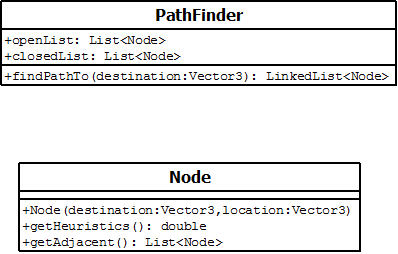
\includegraphics{images/Astar.png}
				\end{center}

		\chapter{\textcolor{blue}{Entities and actions}}
			\section{Robots}
				Since we needed enemies for our game, we decided to design it in a futurist style to match our game's story. We decided to go for the basic enemy of every science fiction story or game and created a robot mesh on Blender. The mesh model has simple shapes since our game itself is supposed to be ``Minecraft-like'' therefore cubic-shaped. As for the texture, they were implemented in-game and are also very simple black and white patterns.\\

				Regarding the animations, we did them very simple too; there are only five different animations :
				\begin{itemize}
					\item death \& shooting
					\item turning around
					\item jump \& walking
				\end{itemize}

				However, we faced many problems when trying to export .blend (3D model from blender) to .mesh (Ogre's 3d format). We even tried using 3DS-max which is another 3d modeling software.Implementing the animations wasn't a simple task either since the tool are too ``old'' and not always compatible with the current software we are using. We struggled to export them and still have some bugs. One of the main issue we had is that every annimations were merged in a single one.
				\begin{center}
					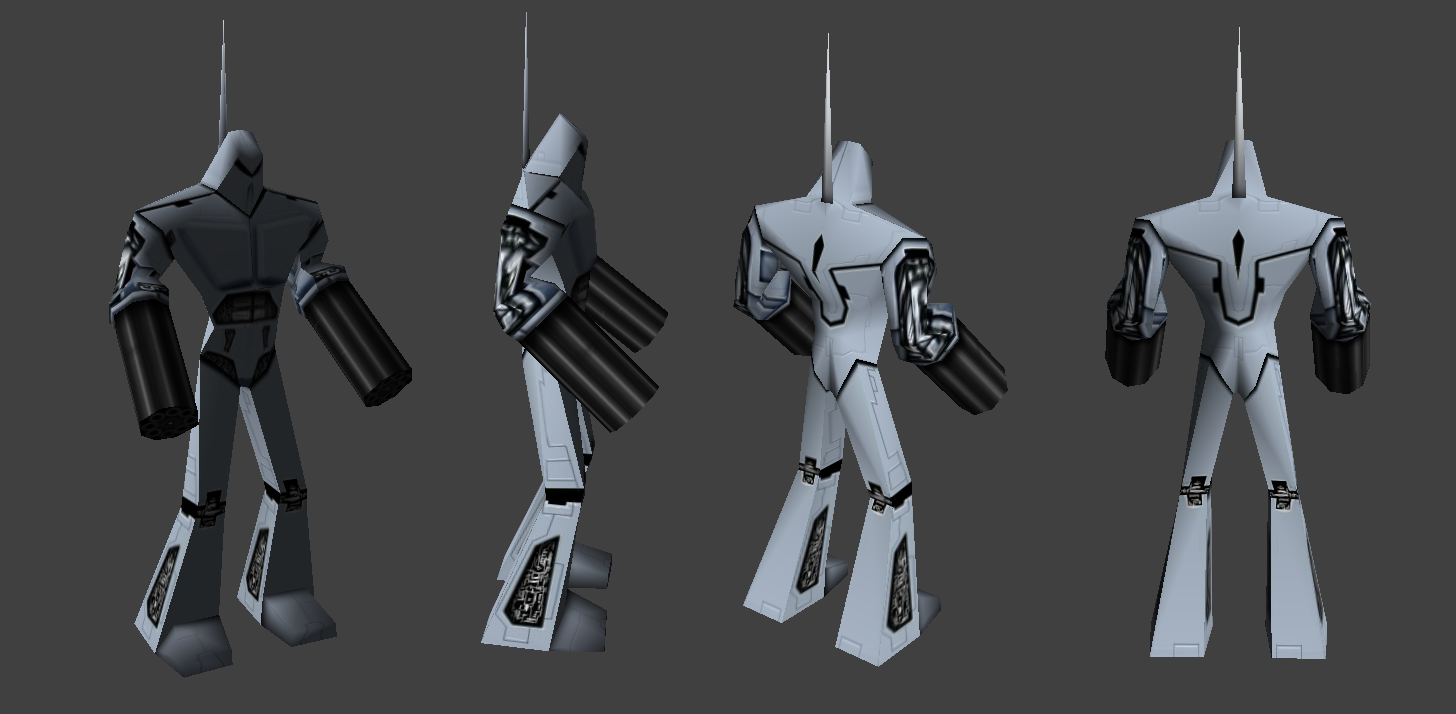
\includegraphics[width = 15cm, height = 4cm]{images/robotMesh2.png}
				\end{center}

			\newpage
			\section{Shooting}
				We have two different shoot system for the AI and the player. The one for the AI is really simple whereas we wanted something more enjoyable for the player.


				\subsection{For the AI}
					When an entity moves and change it's block position, it will get each units in a radius of 16 blocks and tell them it's here, the AI will then move and attack if there is a player in it's reach. Shooting an ennemy is really simple, you just have to create a bullet in front of the entity, give it a good direction using quaternions (a 4 dimension vector which helps representing rotations in 3d) and translate it along the x, y and z axis.\\

					We then need to check the collisions, the basic idea is to cast a ray from the bullet's head to the adverse entity and then check if there are obstacles in between. However, we aren't doing this at each fram for two reasons:\\
					\begin{itemize}
						\item On the one hand to save some precious fps, as you can guess when there will be many AI on the field the fps will decrease a lot so we're already thinking of this matter.
						\item On the other hand, this makes our AI looks more humans. Obviously we, poor little creatures, can't process all the information on the screen each frame. So we try to be fair, we don't want the AI to be invincible.
					\end{itemize}
				\begin{center}
					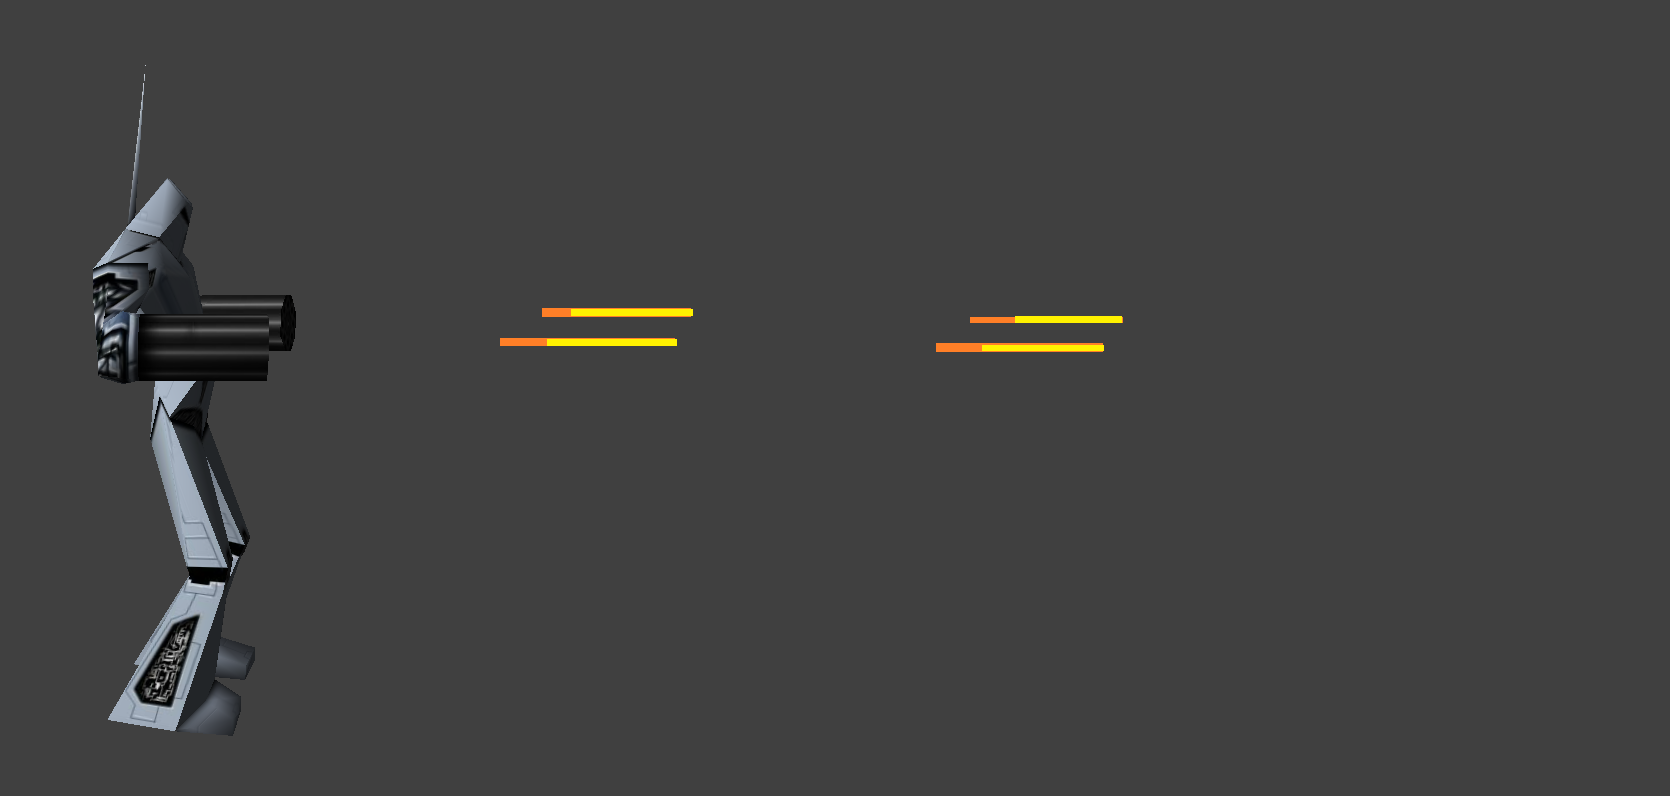
\includegraphics[width = 15cm]{images/robotShoot.png}
				\end{center}
				
				\newpage
				\subsection{For the player}
				\begin{textblock}{0.508}(0.120, 0.15)
					The player's shooting system is very different from the bullets fired by the AI. He doesn't use guns but fireballs, waterBalls or even magicBalls. \\

					To fire them the player must hold the left mouse button down to create a fireball in front of him.
 				It will grow while the button is pressed and will be thrown if the max size is reached or if the button is released.\\
				\end{textblock}

				\begin{textblock}{0.628}(0.630, 0.125)
					\begin{figure}
						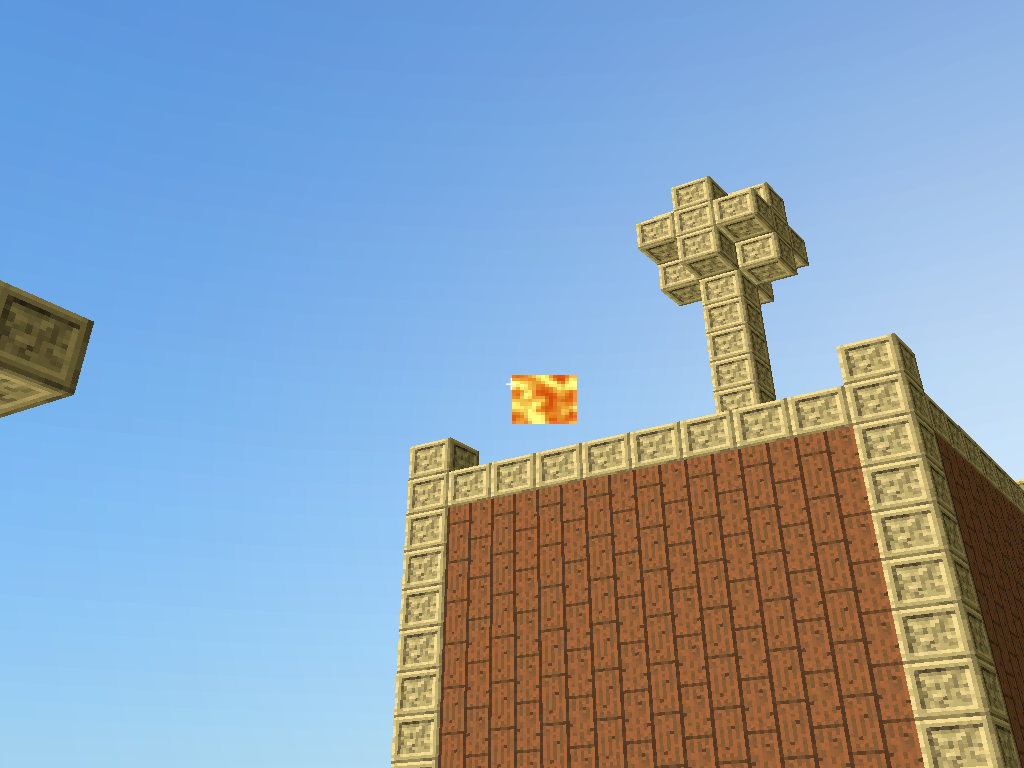
\includegraphics[height = 5cm]{images/Fireball.png}
					\end{figure}
				\end{textblock}
				
				\begin{textblock}{0.628}(0.74, 0.31)
					\it A small fire ball
				\end{textblock}
				
\bigskip\bigskip\bigskip\bigskip\bigskip\bigskip\bigskip\bigskip\bigskip\bigskip\bigskip\bigskip\bigskip\bigskip\bigskip

					We implemented different robot types and thus set their resistance to the different fireballs. Indeed the waterBalls have more damage on fiery robots wherease fireBalls do normal damages against them.\\

					As for the collision, the algorith used to test when an entity is hit is the same as the algorith used for the bullets Of course the bigger the fireball the more damage it will inflict.\\

					Even thought this is a simple idea, we think it improves the gameplay. In a way it let more options to the player to choose how to kill the enemies.

					\begin{figure}[h]
								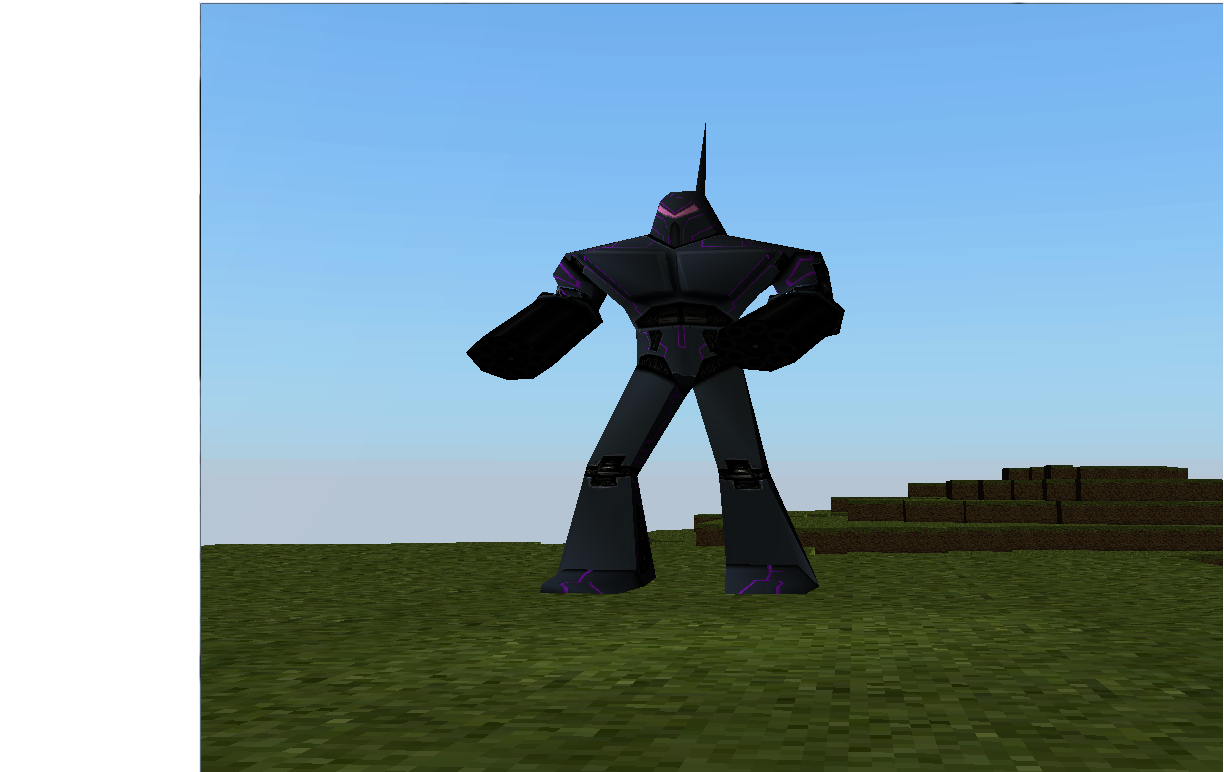
\includegraphics[width=15cm]{images/DarkRobot.png}
								\begin{center}\it A dark robot\end{center}
							\end{figure}
		
		\chapter{\textcolor{blue}{The global AI}}
				To control the the ennemies such as the robot, we implemented what we called a ``global AI'' the basic idea is to thread only one AI which will then compute how much unit it should spawn, where it should move it's units how much ressources it needs to collect.\\

				The IA implemented is very simple and plays according to the players moves. Actually it cheats because it has access to the players stats such as how much units or how much ressources he has. Also, when the AI detects one of the player's unit within 16 blocks of one of it's units, the AI sends units to check if the player is trying to attack it and, if this happens he usually tries to send his whole army there.\\

				Of course this is not the AI used for the dark tower because in the dark tower, there is no base and thus the unit cannot be respawned nor can they gather ressources. Therefore the AI manage the units floors by floors, when they detect a player, they gather and attack him.

				\begin{center}
					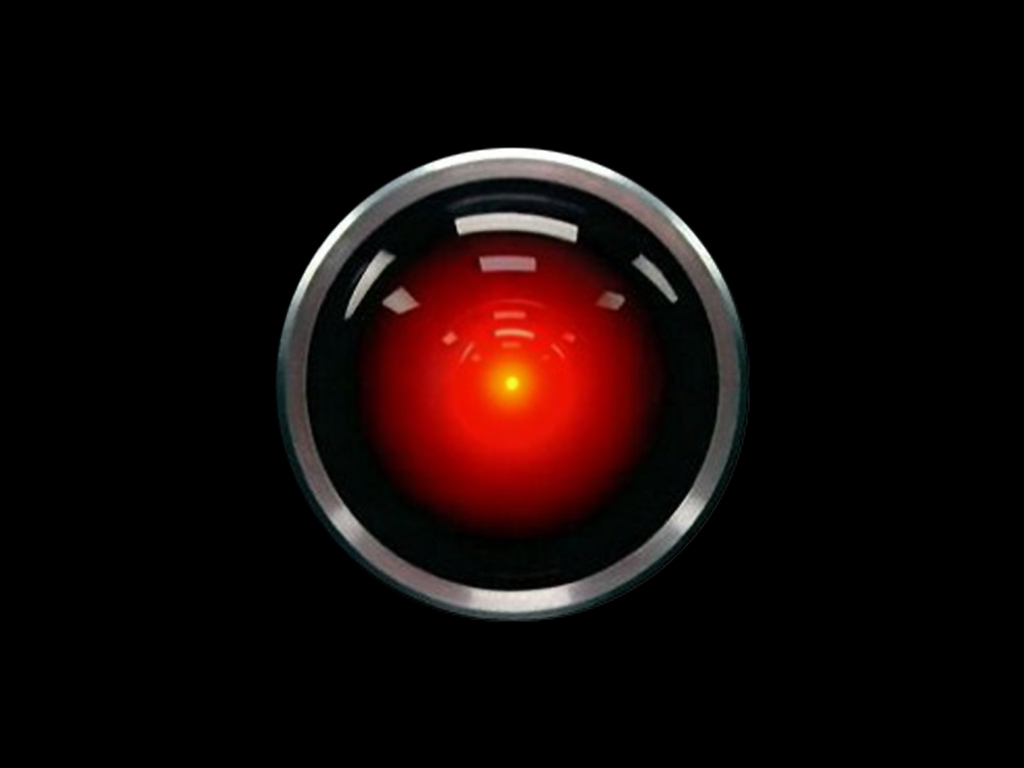
\includegraphics[width=15cm, height = 10cm]{images/hal.jpg}
				\end{center}

		\chapter{\textcolor{blue}{Saving and Loading the game}}
			\section{Algorithm}
				Saving and loading the terrain were mostly done at the last oral presentaion. However since we implemented other entities, we had to save and load them as well.
				As you know each different block possess an id (for example the id of the grass blocks is  1) which is stored in char whose weight is only one bite. Therefore we can store the terrain pretty easily, the 3 first bites beeing the terrain's size and the others beeing the blocks id stored in the x, y, z order.

				This time, for the entities we choosed the easy way, registering the id of an entity and its position next to one another. Just like this:\\						
							\begin{center}
								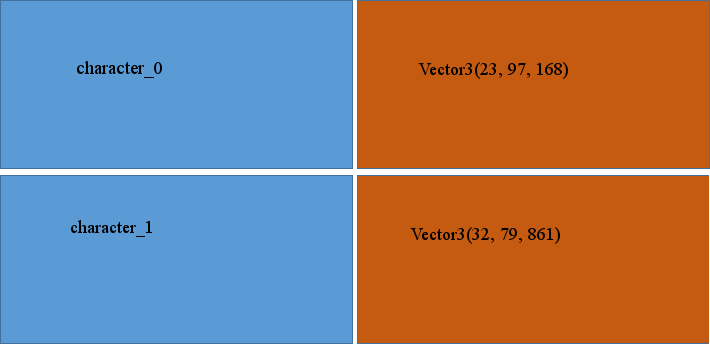
\includegraphics[width = 15cm]{images/Save.png}
							\end{center}
				
				One of interresting thing with this method is the fact that the id which is an byte stores more than one information. Because a byte can store a number up to 255, this means it is composed of 8 digits (0000 0000), using a system of mask on the binary value we can actually store 2 information.

				For example : 
				\begin{lstlisting}
					byte a = 0xF3; //1111 0011 in hexadecimal
					Console.WriteLine(a & 0xF);//Outputs 0011
					Console.WriteLine((a >> 4) & 0xF);//Outputs 1111
				\end{lstlisting}

			\section{A new menu}
					With the save and load algorith, we felt that our old menu wasn't adapted to the mindset we had for this game. We didn't want the player to be able to choose what Island he could go on or what size! This menu was intended for debug purposes not for ou final product.\\

					So, in order to adapt the old menu to the mindset we thought of and to add an adventure mode to the game, we decided that the player would only be able to create one world and choose to either continue the last world he created either create a new one, removing the last one he made.

			\section{Integration to the menu}
					As I've already said, the menu we had was intended for debug purposes only. Our idea for this menu was to let him create only one world and then to let him choose between 


		\chapter{\textcolor{blue}{Structures}}
			\section{Behind the scenes}
				Handling the structures was an easy task therefore, we decided to complexify it, making it easier to implement more than one structure at a time. The basic idea was to not just have multiple list of structures in the island class and then have a switch which would choose the list according to the biome.\\

				After thinking about a little bit we decided to make use of the inheritance via the abstract Biome class which implemented the methode populate calling the list of structure which is contained in every derived class of Biome.
				\begin{center}
					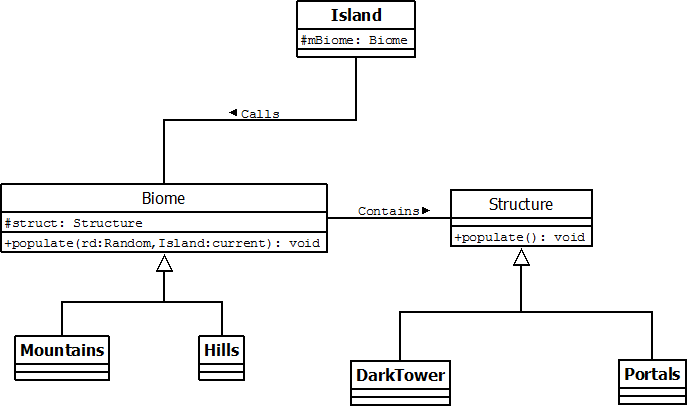
\includegraphics[width=15cm]{images/Structures.png}
				\end{center}
				\newpage

			\section{Portals}
				One of our goal for this oral presentation was to establish a link between the islands to ensure the continuity of the game. Therefore we created the portals, they one island to another.\\

				Of course they are structures and are derived from this class and were generated procedurally. At the moment, the game has two types of portals a ``door'' and a ``pool'' and they can have a red, green or blue texture : 
				\begin{center}
					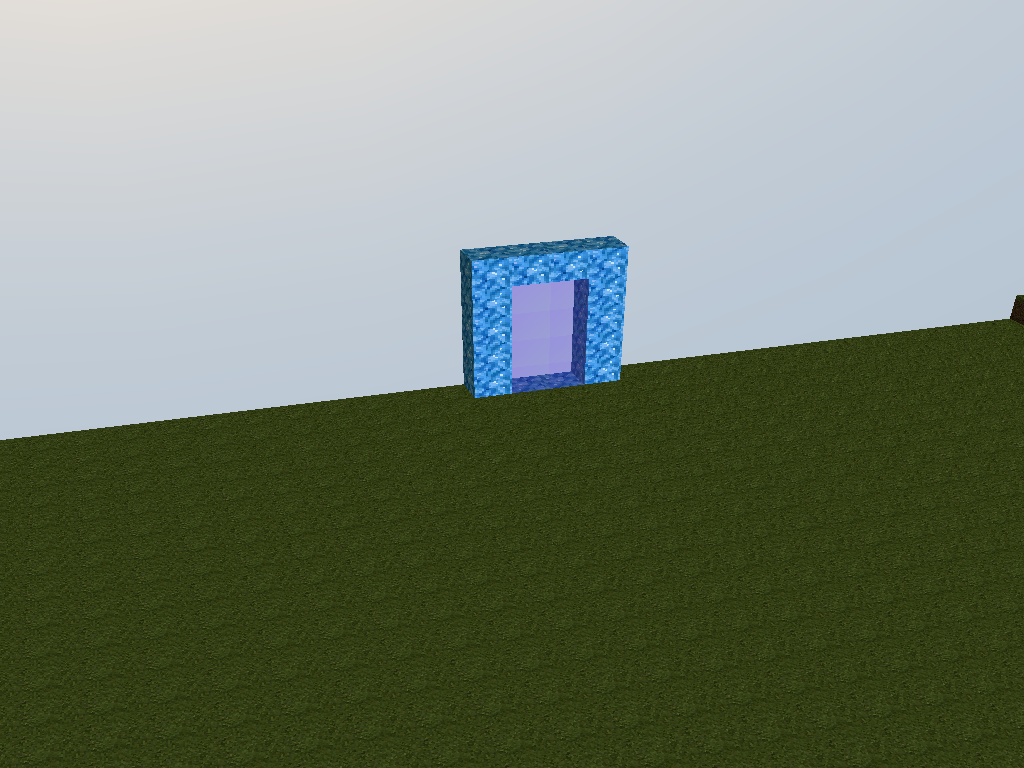
\includegraphics[width=7.5cm]{images/Portal1.png}
					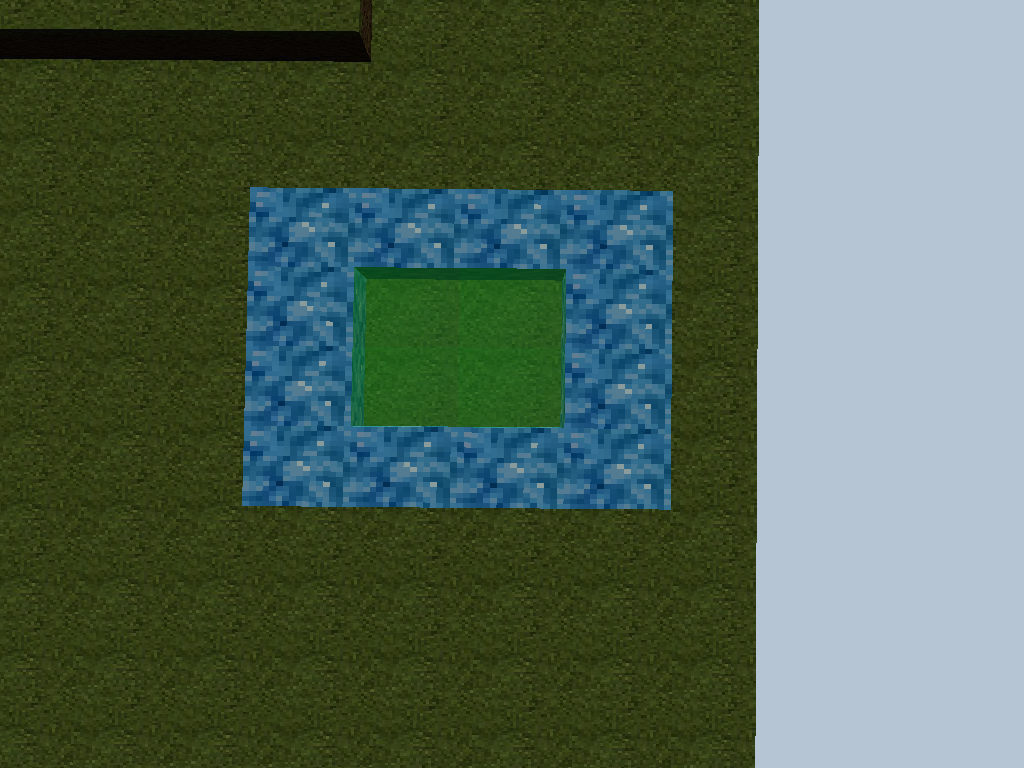
\includegraphics[width=7.5cm]{images/Portal2.png}
				\end{center}

				When the player performs an action such as moving from one block to another, right clicking on a block, left clicking, creating or even destroying a block he triggers an event. In our case, we use the onBlockEnter event which is in the Block class and overrided by some classes. Basically, when an entity enters the portal, it is teleported to island which it's connect.
			\section{Buildings}  
				Unlike the previous oral presentation this time we have multiple buildings. Some were generated as a ``bunker'' for the portals just like the dark tower or the pyramid and others were designed to perform specific task such as the magician's tower or the infantry portals. Until now we generated the following structures :

				\begin{center}
					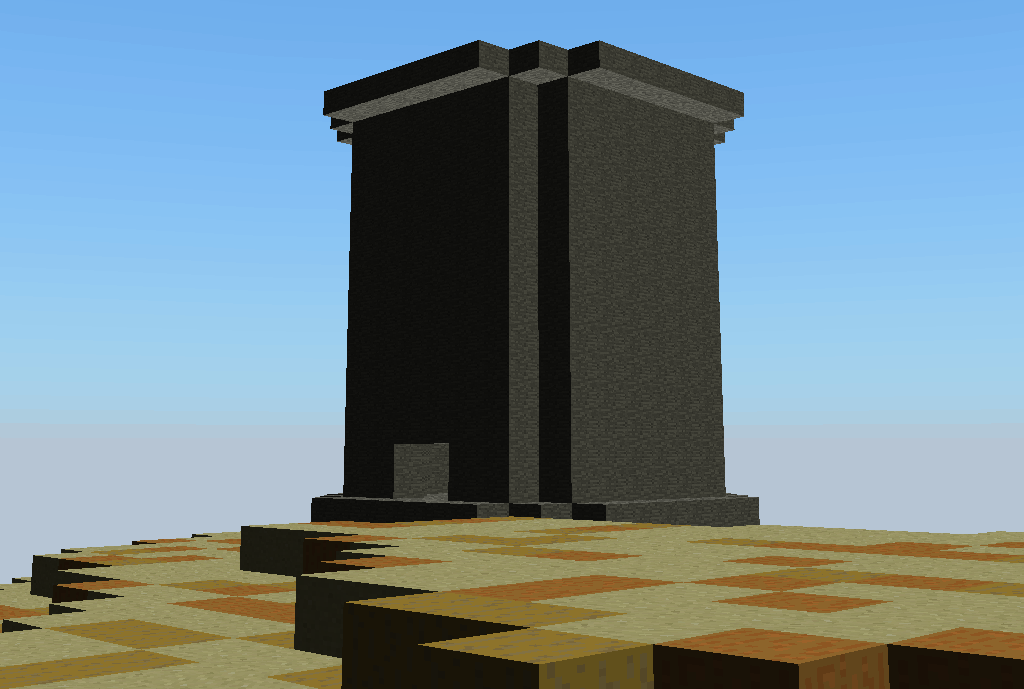
\includegraphics[width=5cm]{images/structure.png}
					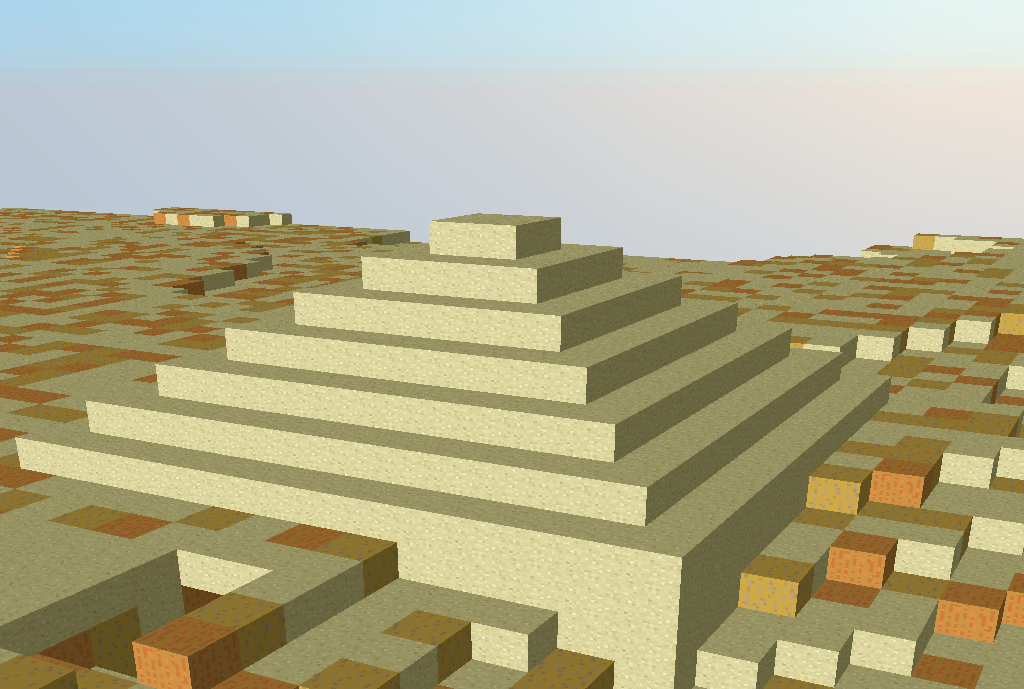
\includegraphics[width=5cm]{images/structure2.png}
					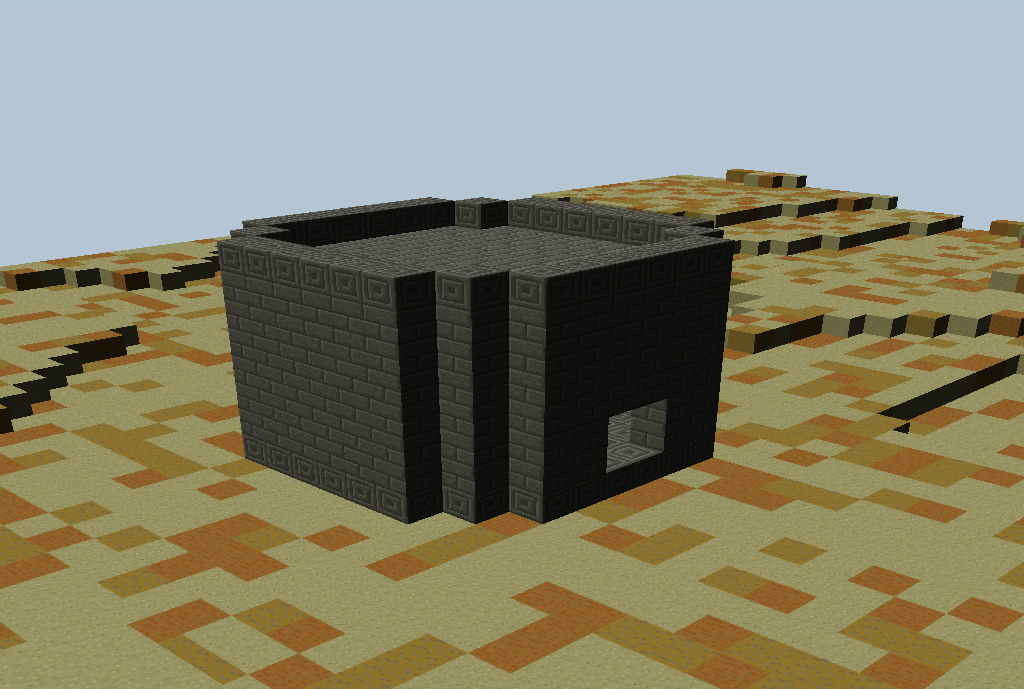
\includegraphics[width=5cm]{images/structure3.png}
				\end{center}
				
				As you already know, the structrures are derived from the abstract base class strcture and are generated procedurally. Creating them was a particullarly boring part of the creation of this video game but we managed to have some cool results.\\



		\chapter{\textcolor{blue}{The dark tower}}
			\section{Introduction to the dark tower}
				The dark tower is the biggest structure we made, it is composed of four main towers floating in the sky and is part of the plain biome. This structure is huge because it size can reach 362 blocks on the y axis and has almost 41 floors


			\section{The main buildings}
				The tower consists in four main buildings whose height vary between 60 and 88 blocks it has about seven floors which can be climbed using the arcane levitator which as it names implies allows you to levitate. Basically if you are on the levitator, it will lift you up to the next floor.

				\begin{center}
					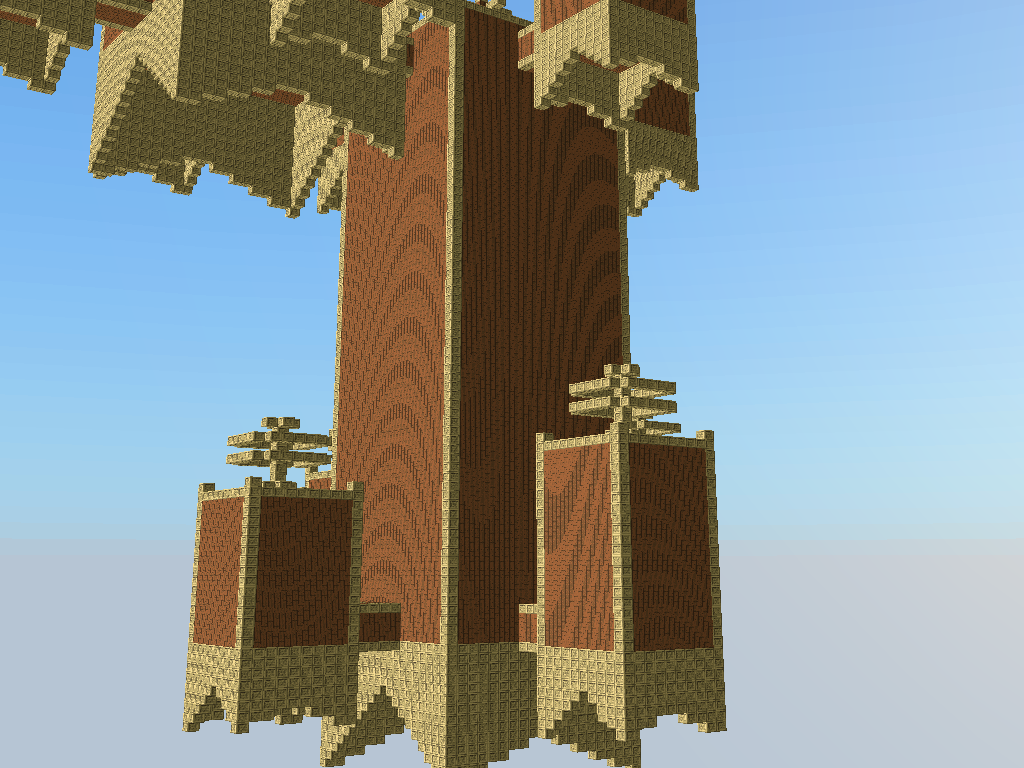
\includegraphics[width=7.5cm]{images/DT/Main.png}
					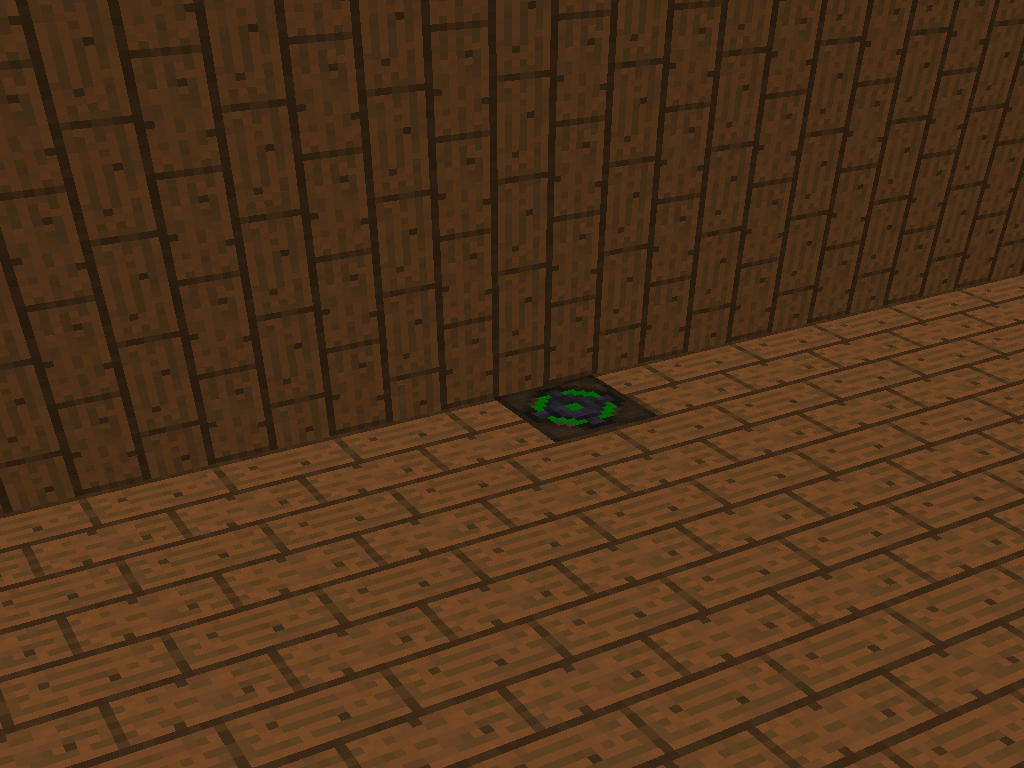
\includegraphics[width=7.5cm]{images/DT/floor.png}
				\end{center}
			finally on the first and last floor of the main tower, bridges connect the main towers to medium towers or another main tower.

			\section{Bridges}
				Bridges are generated only by the main towers and allows the player to continue climbing the dark tower. One difficulty we encountered while ``building'' the tower was the orientation. Indeed, the algorith to build a bridge facing north is not the same as the algorithm to build a bridge facing west. We struggled to find a way to ``unify'' those algorithm but we finally choose the simplest solution using a switch. Here is the result :
				\begin{center}
					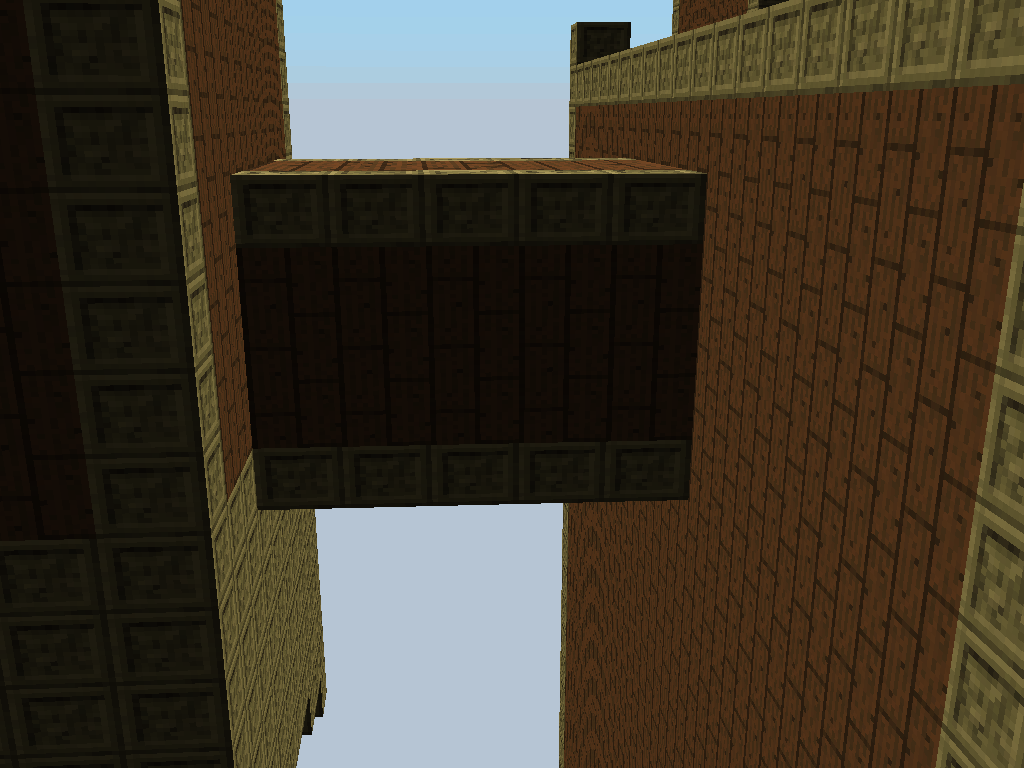
\includegraphics[width=7.5cm]{images/DT/bridge1.png}
					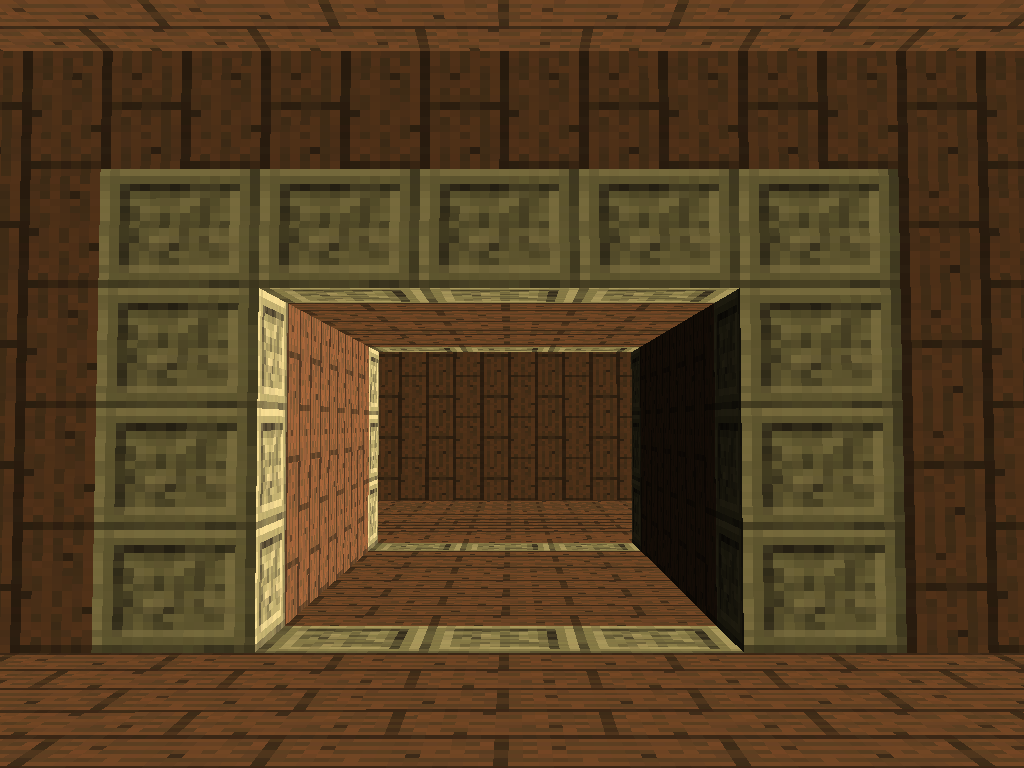
\includegraphics[width=7.5cm]{images/DT/bridge2.png}
				\end{center}

			\section{Lower towers}
				As I've already said before the main tower are linked by bridges to lower towers their height vary between 15 and 30 blocks and in most of them, the player will find prisonners unit guarded by ennemies and when they are defeated (the ennemies), the prisonners joins the player which can then command them.
				\begin{center}
					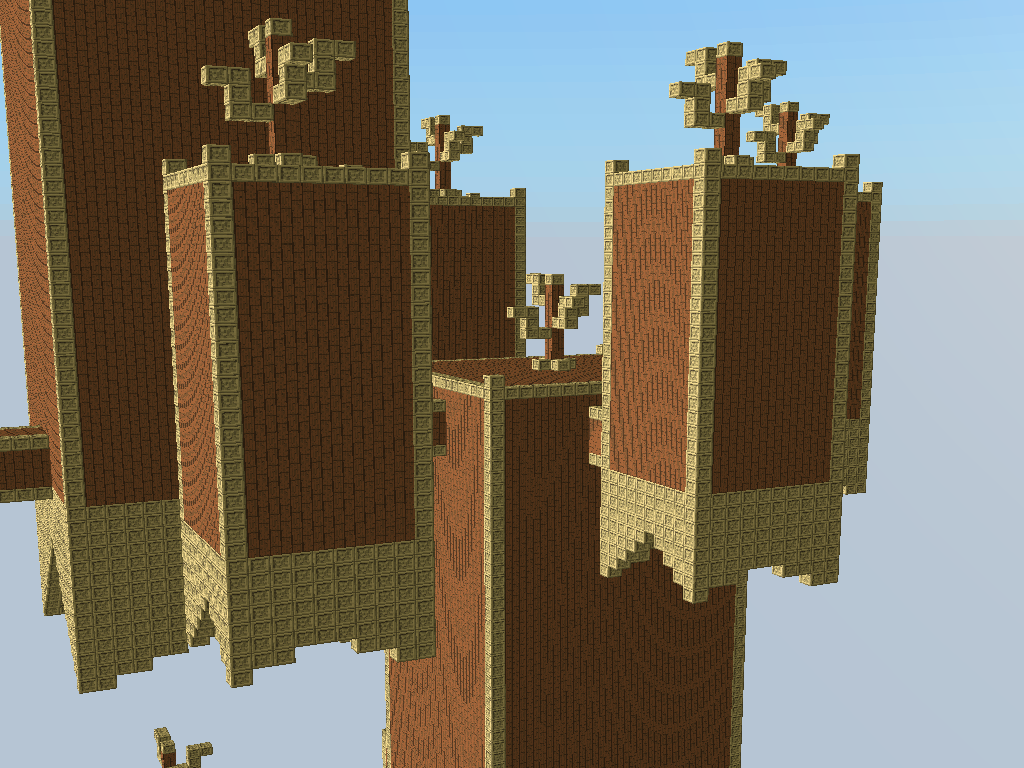
\includegraphics[width=7.5cm]{images/DT/mediumTowers.png}
					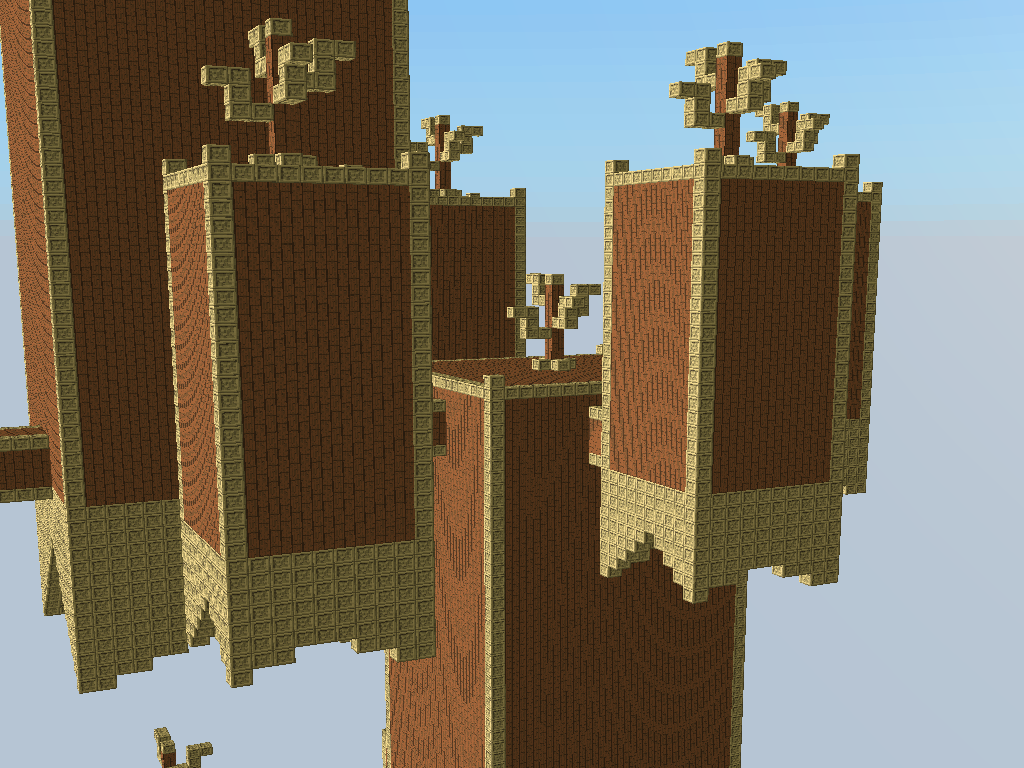
\includegraphics[width=7.5cm]{images/DT/mediumTowers.png} %TODO : Robots
				\end{center}

			\section{Roofs}
				Among the multiple things which make the tower, one of the most beautiful thing are the structures on the roof, we made 3 of them :
				\begin{center}
					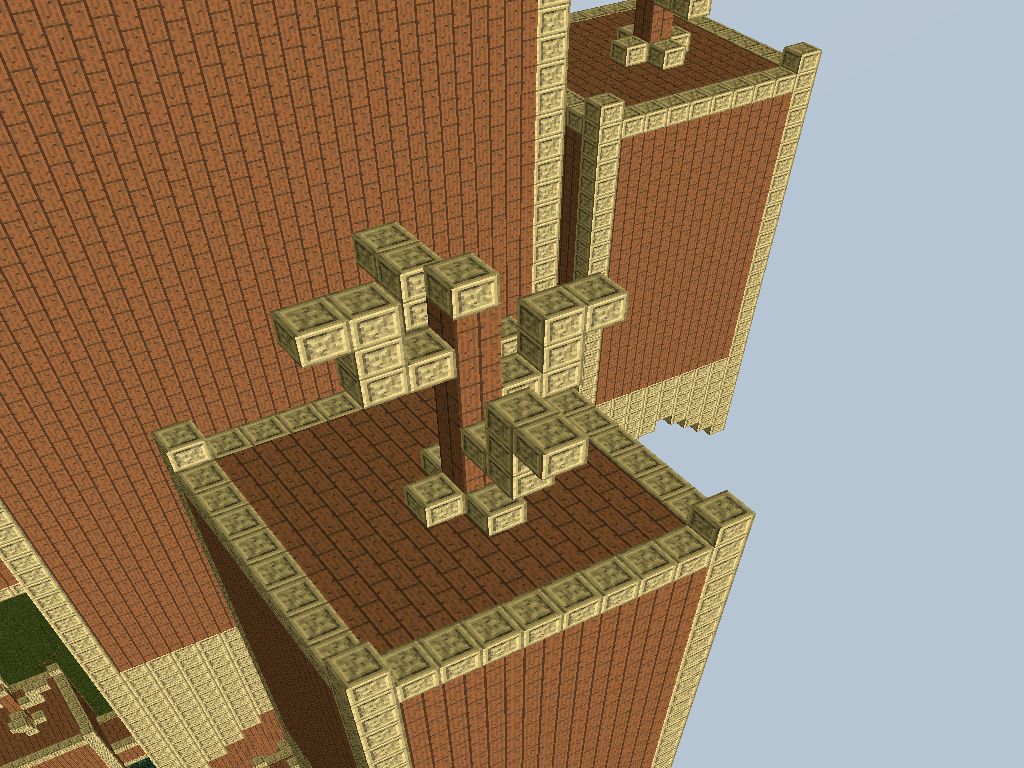
\includegraphics[width=5cm]{images/DT/roof1.png}
					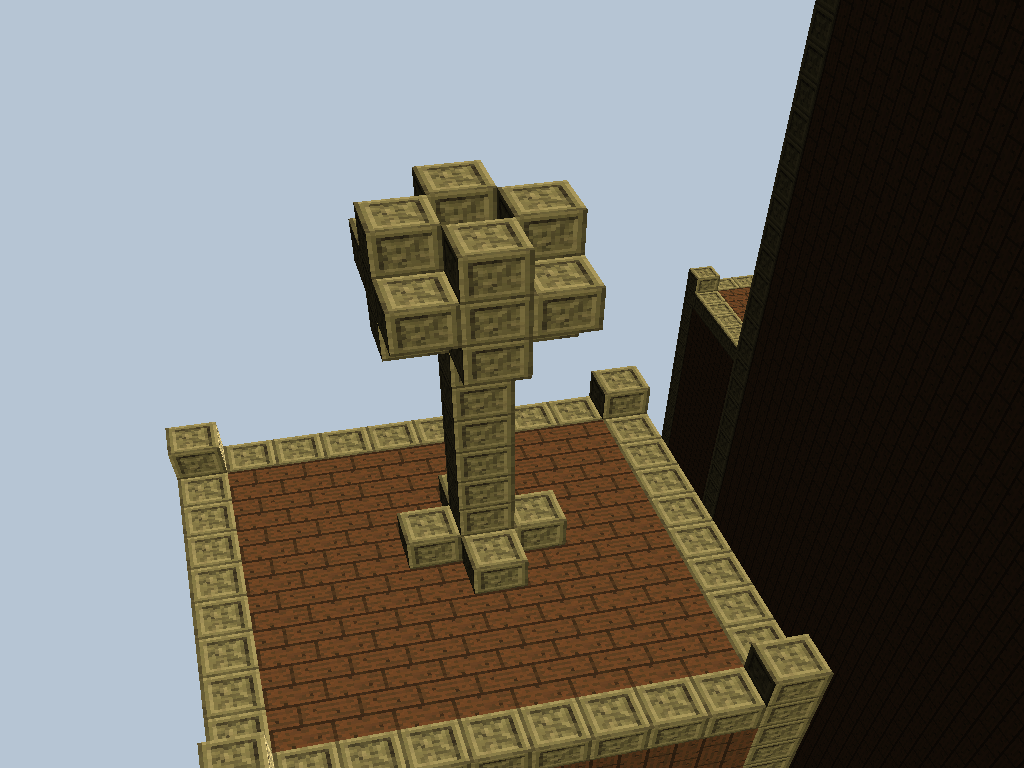
\includegraphics[width=5cm]{images/DT/roof2.png}
					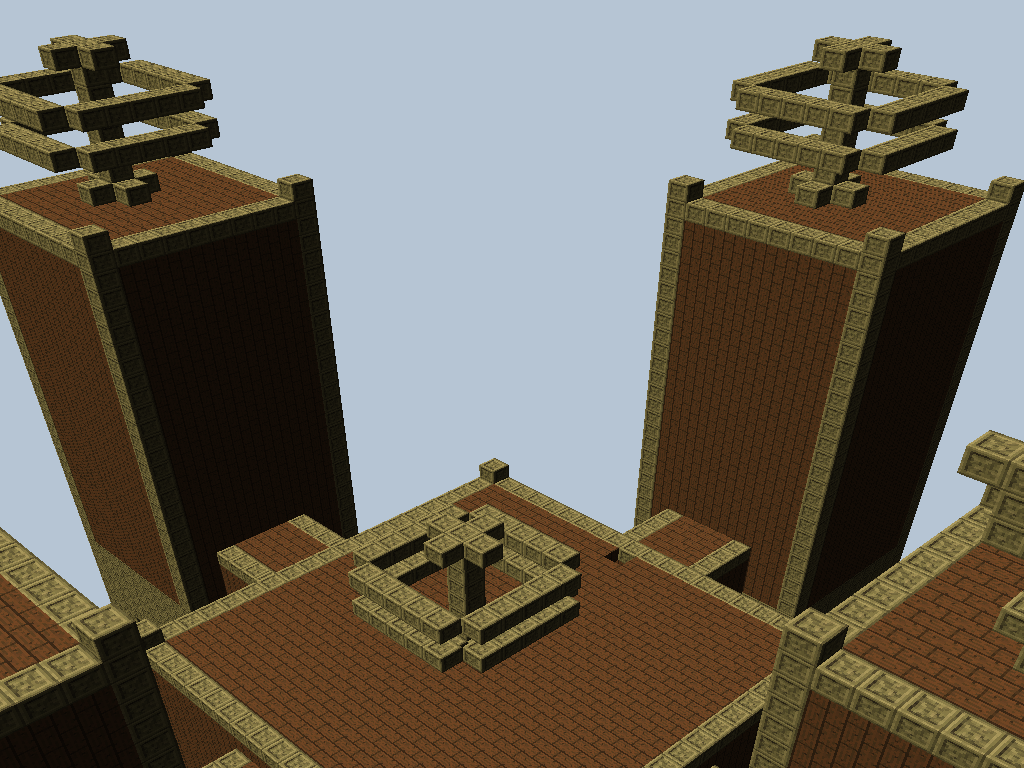
\includegraphics[width=5cm]{images/DT/roof3.png}
				\end{center}


			\section{DarkBeard}
				Finally, we had to deal with the bottom of the towers. At the beginning we thought that it would stay flat but, we managed to find a function that made the bottom look amazing. We called it the dark beard.

				\begin{center}
					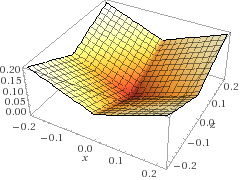
\includegraphics[width=7.5cm]{images/Abs.png}
					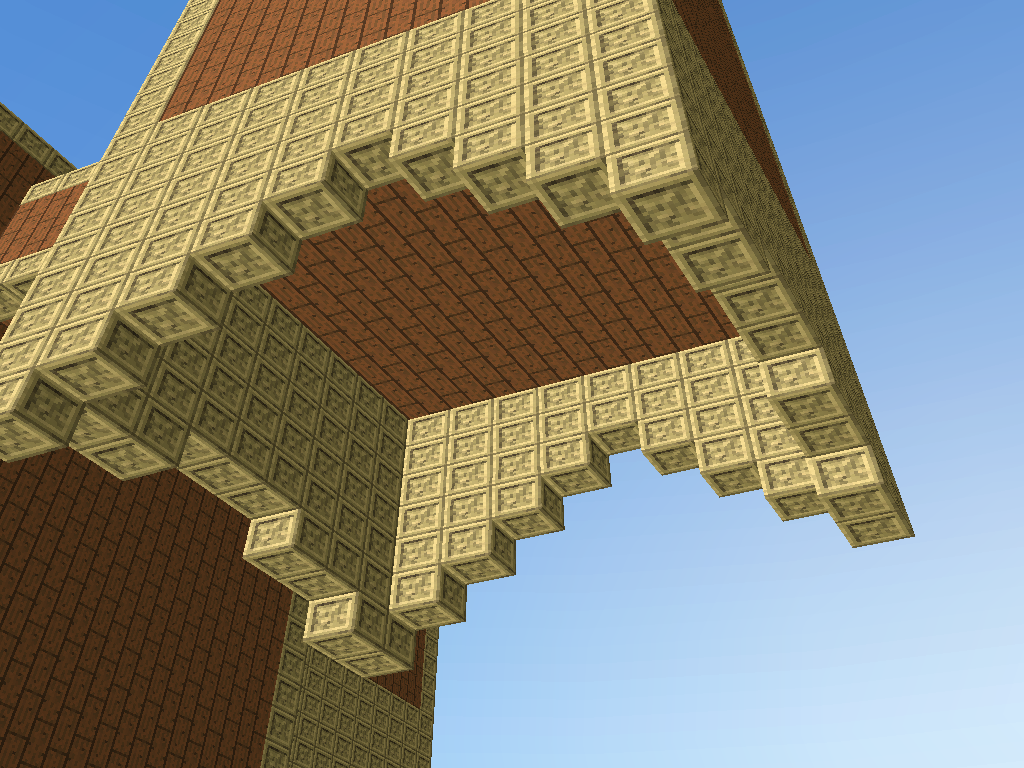
\includegraphics[width=7.5cm]{images/DT/DarkBeard.png} %TODO : Robots
				\end{center}

		\chapter{\textcolor{blue}{Graphics}}
			\section{Shadows}
				As you might have seen, our game did not have any shadows, thus we decided to implement some. After a long period of testing, we discovered that integrating real shadows in the game would cause an enormous drop of FPS which ended up crashing the game, no matter what we did.\\

				Therefore we settled for an intermediate solution, shadows are beeing calculated on the mesh only once, at the begining thus giving a better result than a game without shadows.

				\begin{center}
					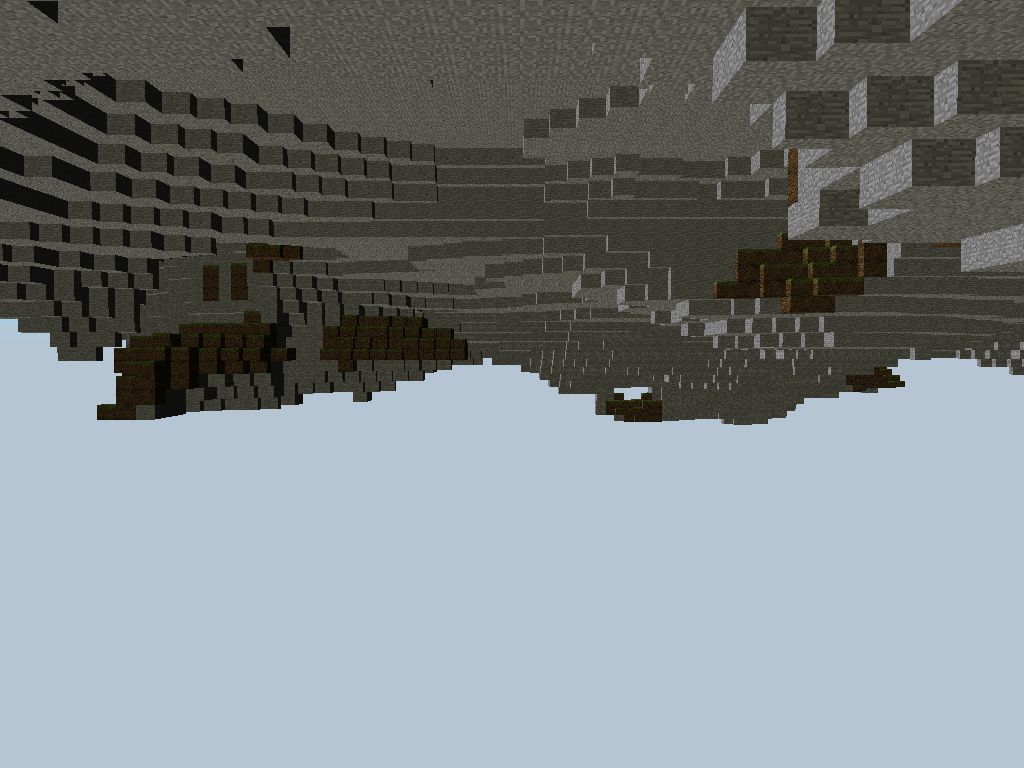
\includegraphics[width=8cm]{images/shadows.png} %TODO : Robots
				\end{center}
					\begin{textblock}{0.575}(0.110, 0.785)
					As you can see here, some faces are darker than others, and one is unexpectedly bright, the ``lower'' face this is because the planet is only composed of skylands and thus, the light also comes from under the terrain.\\

					To set the shadows, we had to set normals and, at first we were confused, because we were told to use the cross product to compute the normal's value. Then after thinking a bit about it, we discovered that the only normals we needed were simple and didn't need to be calculated, we could simply add them to the code....
				\end{textblock}

				\begin{textblock}{0.628}(0.690, 0.75)
					\begin{figure}
					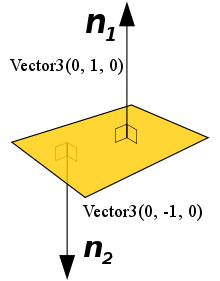
\includegraphics[width=5cm]{images/normal.png}
					\end{figure}
				\end{textblock}
\newpage
			\section{Having fun with textures}
				\begin{textblock}{0.628}(0.130, 0.16)
				\begin{figure}
					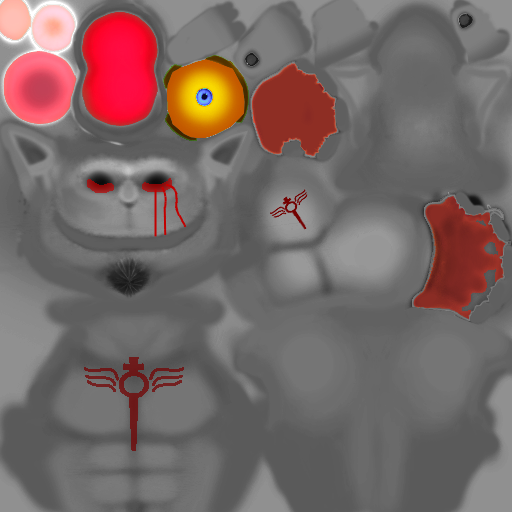
\includegraphics[width=5cm]{images/sinbad_body.png}
				\end{figure}
				\end{textblock}
				
				\begin{textblock}{0.575}(0.40, 0.2)
					Creating a whole mesh and all its animation is not always possible. Modifying the texture thought is different. You casn see on the left a .tga files. They are used to apply textures to 3d models. But how can we apply a 2d image to a 3d image ? This is what we called the UV mapping and that's a really powerfull technique.
				\end{textblock}
				
				\bigskip\bigskip\bigskip\bigskip\bigskip\bigskip\bigskip\bigskip\bigskip\bigskip\bigskip\bigskip\bigskip\bigskip\bigskip\bigskip\bigskip
				
				We can do the same for the robot mesh. We will use these different textures to distingue each factions. You can see below 2 different textures for the robots. If you wan to see the result on a 3d model, well you will have to turn the page.
				
				\begin{textblock}{0.628}(0.120, 0.47)
					\begin{figure}
						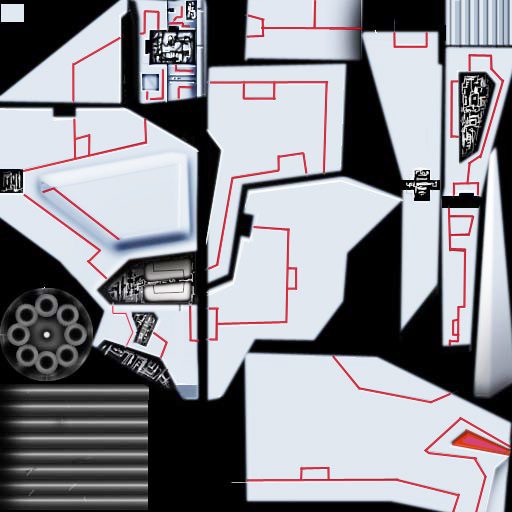
\includegraphics[width=6cm]{images/r2skin_K.jpg}
					\end{figure}
				\end{textblock}
				
				\begin{textblock}{0.628}(0.58, 0.47)
					\begin{figure}
						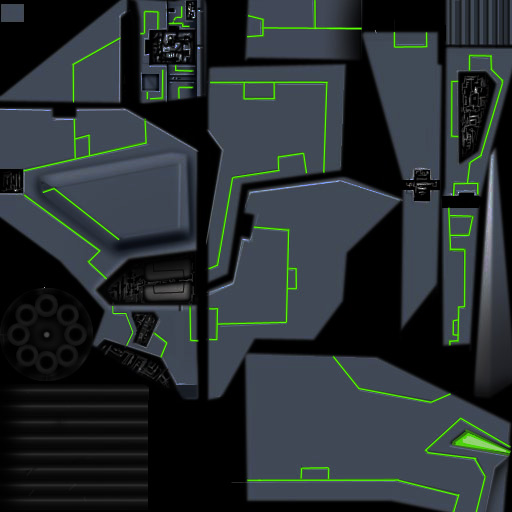
\includegraphics[width=6cm]{images/r2skin_T.jpg}
					\end{figure}
				\end{textblock}
				
				\newpage
				
				
				\begin{center}
				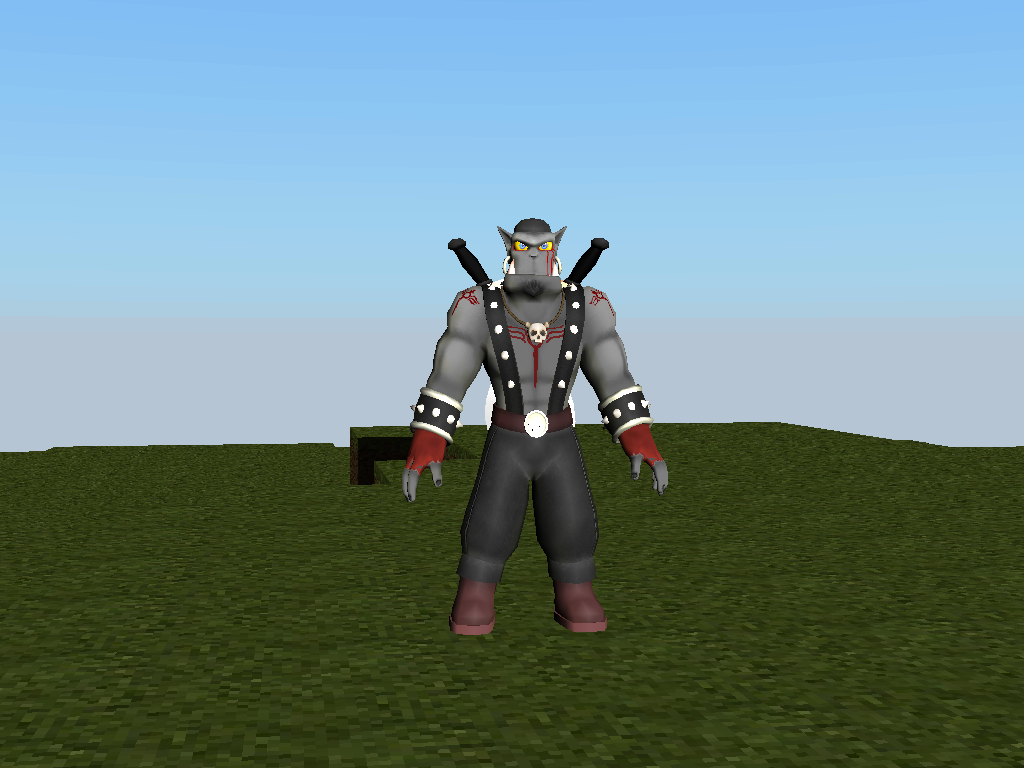
\includegraphics[width=14.5cm]{images/newSinbad.png}\\
				\it The new Sinbad
				
				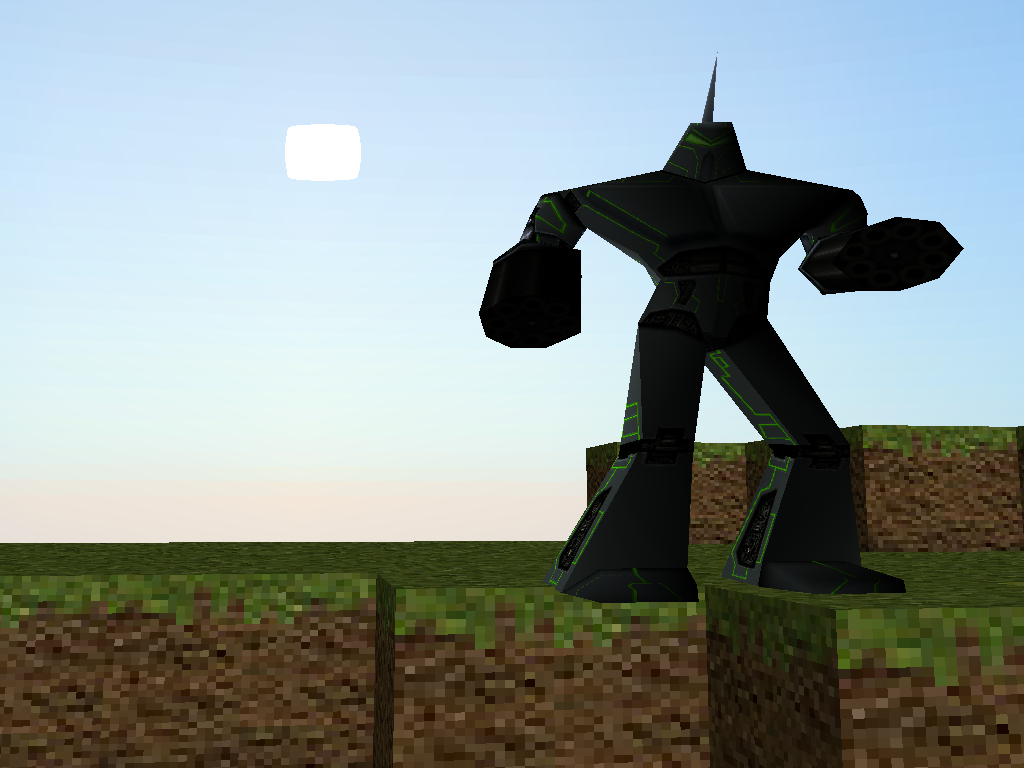
\includegraphics[width=14.5cm]{images/greenRobot.png}\\
				\it A green robot
				\end{center}
				
				

		\chapter{\textcolor{blue}{Conclusion}}
			Unfortunately you have reached the end of this marvelous report! As you've seen throughout this report, we have worked very hard for this oral presentation. The result talk for themselves and the goal fixed were reached.\\
			
			Most of the game is still a work in progress (WIP), much has to be done in little time. However, the team is still standing and ready to work on those things !
			
			
\end{document}